\section{Results}
\label{sec:perovskites-results}

%\bit
%\item Stabilisation confirmed via dimer calculations
%\item Ridge calculations performed and their results are ...
%\item Ridge calculations performance on a production DFT system
%\item Hard to say if medium range stabilisation takes place (outlook: do similiar calculations using larger cells)
%\eit

\subsection{Confirming Previous Results}
The results of \cite{double-defect-2011} showed that the hydrogen atoms would move in individual steps while staying close to each other.
Two such mechanisms were discussed and both consisted of multiple iterations of two types of events.
Either the transitioning hydrogen atom would "jump" from one oxygen atom to the next near a titanium atom or it would "rotate" past a strontium atom while remaining near the same oxygen atom.
Both hydrogen atoms would perform these steps --- often in alternating order --- while remaining in close proximity of each other.

Dimer \sap{1} searches were conducted, starting from the various minima suggested in \cite{double-defect-2011}.
Essentially, confirming the previous results, the low energy \sap{1}s were all events of the types described above.
Only a handful of truly concerted events, where both hydrogen atoms would transition simultaneously, were detected but they were all higher in energy.

Some \sap{1}s were found at a slightly longer range, e.g. where the hydrogen atoms would be separated by a strontium atom.
In the calculational cell used this is effectively half of its length, bringing into question any discussion on the energies as periodic effects could both over- and underestimate the stabilisation by the neighbouring hydrogen atom.
Further investigation of these might prove interesting but a larger calculational cell is required.

\subsection{DFT Ridge Calculations}
The same parameters were used for the dimer part of the ridge calculations as were used for the dimer searches above.

A few ridge calculations were started with some of the \sap{1}s found above as endpoints.
The general results can be split into three categories.
\bit
\item Successful ridge calculations, converged from a linear interpolation to a ridge in under 300 iterations.
\item Calculations where a soft eigenmode was followed resulting in a non-converging calculation where the lattice would distort heavily.
\item Unsuccessful calculations where the path would spent most of its time as an inverted barrier near the minimum energy path.
\eit

The most interesting of the successful ridge calculations was one where the environment of a jump-type \sap{1}s consisted of a rather flat energy profile with lattice motion before a sharp rise to reach a $0.08\unit{eV}$ \sap{2} on its way to a rotation-type \sap{1} for the other hydrogen atom.
Both the flat energy profile and the low \sap{2} are clear warning signs, that the HTST rate could be improved.
\begin{figure}[htb]
\begin{center}
  \subfigure[The configuration of the A-jump \sap{1}. One titanium atom is semi-transparent to allow viewing of hydrogen B]{
    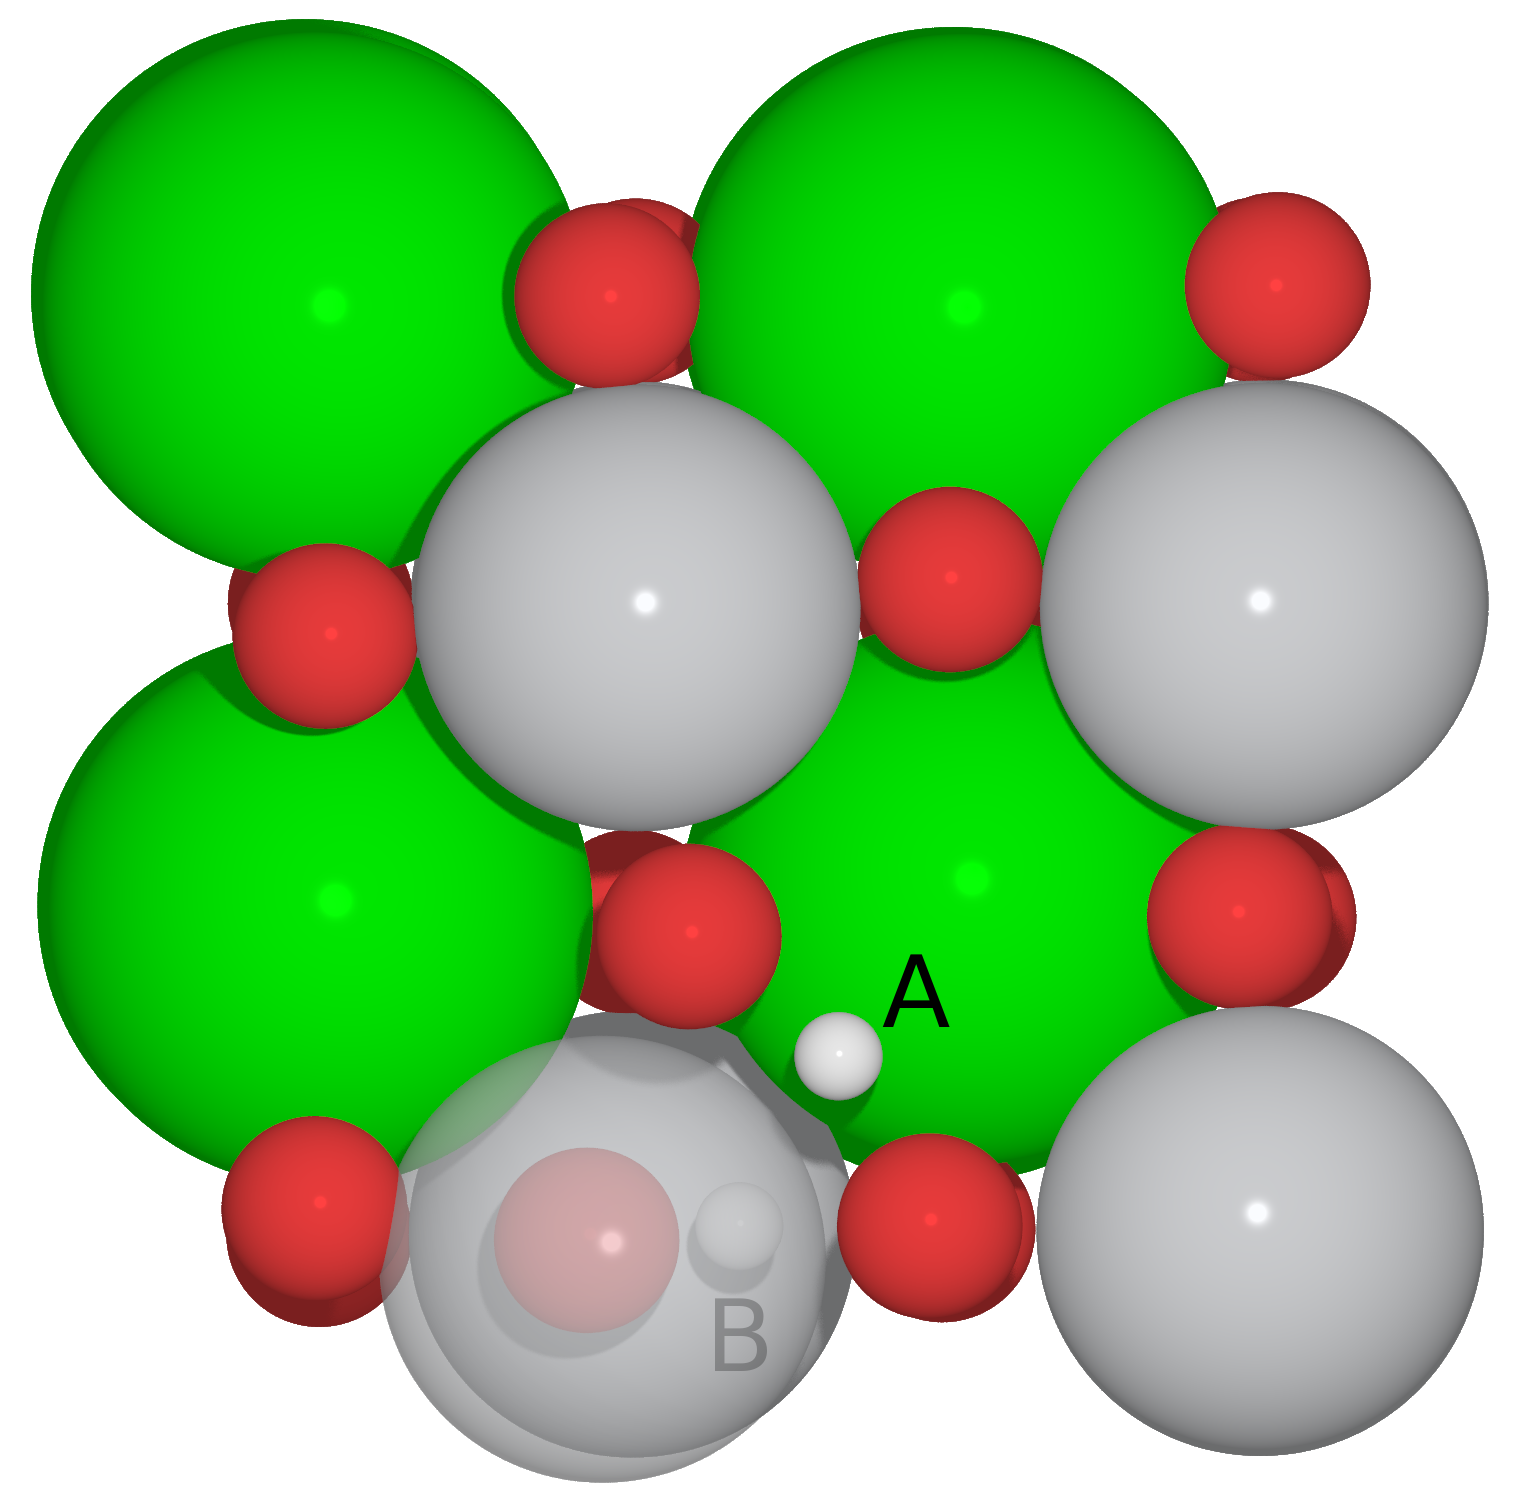
\includegraphics[width=0.45\linewidth]{semi-combined}
    \label{fig:semi-combined}
    }
  \subfigure[Energy profile of the ridge]{
    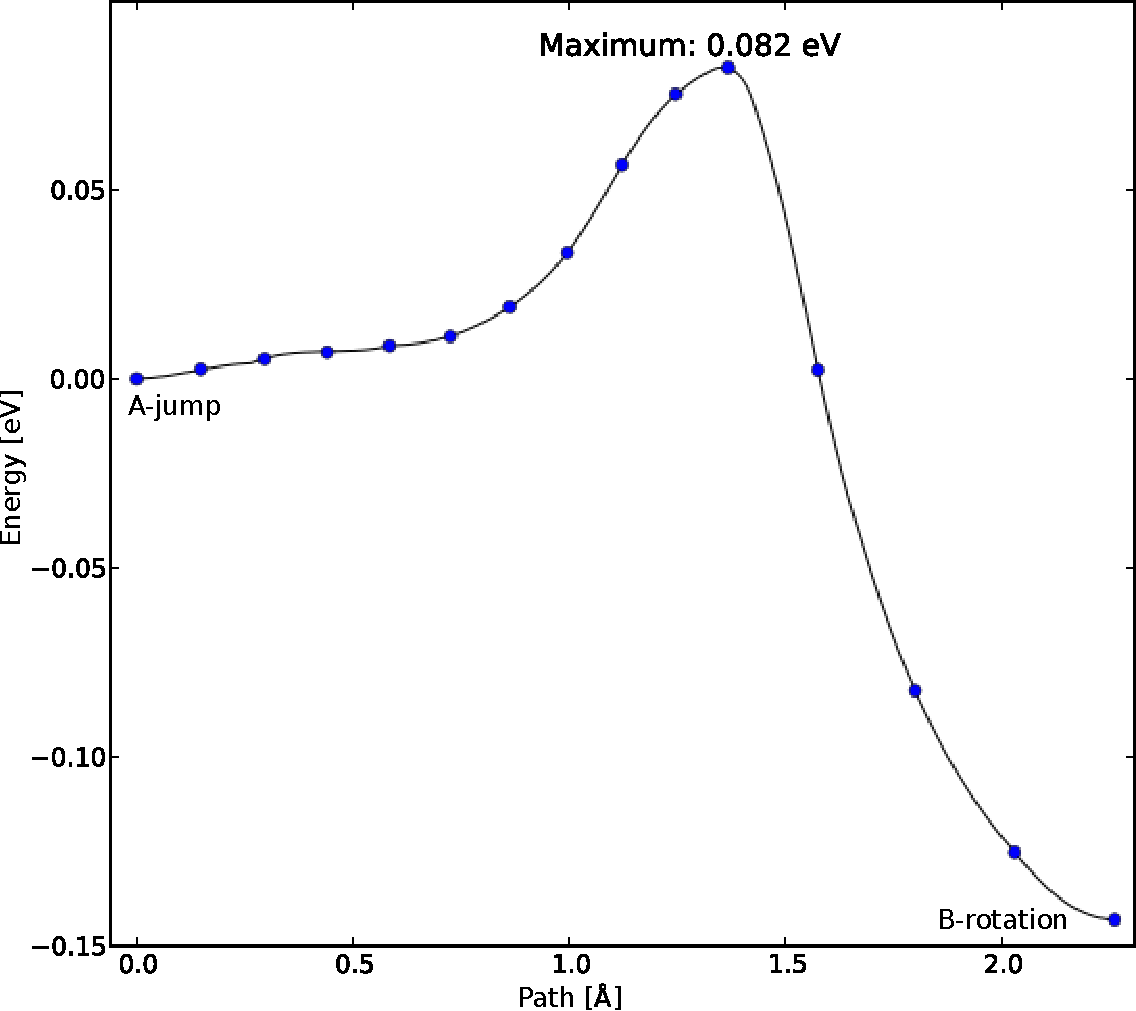
\includegraphics[width=0.45\linewidth]{semi-ridge}
    \label{fig:semi-ridge}
    }
    \parbox{0.85\linewidth}{
      \caption{A successful DFT ridge calculation between a jump \sap{1} for hydrogen atom A and rotation of hydrogen atom B.
The hydrogen atoms are white, the titanium atoms are grey, the strontium atoms are green and the oxygen atoms are red.
      }
      \label{fig:semi-results}
    }
\end{center}
\end{figure}


Latching on to a soft eigenmode is a concern that is always possible with dimer-type algorithms.
However, this was not a significant problem in previous tests.
In this particular case, the climbing image had been turned on very early in order to avoid the basin trapping problem.
After the climbing image is turned with a soft eigenmode, the calculation is unlikely to yield an interesting result.
This problem raises questions about the lack of similarities for neighbouring eigenmodes.
If a random initial eigenmode is used (as was the case in this calculation), is it likely that \expand
This was not a problem for the test systems

Many of the calculations resulted in paths that lay near the MEP and minimum.


%Approximately half of the started calculations reached a ridge under 500 iterations, while the rest struggled.
Those calculations that did not reach the ridge, generally lay near the minimum energy path and were not able to rise out of the basin.
The eigenvalue estimate would remain negative for most of the images.

One calculation latched onto a soft eigenmode where the whole lattice would move.
This is always a danger when using the dimer to find a minimum mode.
\tred{This is particularly dangerous if the CI is used on an image with a bad estimate. There is no check for such a thing.}

Picking the most relevant \sap{1}s as endpoints a few ridge calculations were attempted.
Well behaved cases converged quickly but some would get trapped near minima and spend hundreds of iterations there until the calculations were aborted.
It is unlikely that this minima-trapping behaviour is an artefact of the method itself as such things did not happen in the previous test cases.\footnote{Or did they in the difficult 3-atom vs. 2-atom concerted cases?}



